

\documentclass[twoside,twocolumn]{article}

\usepackage{blindtext} % Package to generate dummy text throughout this template 

\usepackage[sc]{mathpazo} % Use the Palatino font
\usepackage[T1]{fontenc} % Use 8-bit encoding that has 256 glyphs
\linespread{1.05} % Line spacing - Palatino needs more space between lines
\usepackage{microtype} % Slightly tweak font spacing for aesthetics

\usepackage[english]{babel} % Language hyphenation and typographical rules

\usepackage[hmarginratio=1:1,top=32mm,columnsep=20pt]{geometry} % Document margins
\usepackage[hang, small,labelfont=bf,up,textfont=it,up]{caption} % Custom captions under/above floats in tables or figures
\usepackage{booktabs} % Horizontal rules in tables

\usepackage{lettrine} % The lettrine is the first enlarged letter at the beginning of the text
\usepackage{todonotes}
\usepackage{enumitem} % Customized lists
\setlist[itemize]{noitemsep} % Make itemize lists more compact

\usepackage{abstract} % Allows abstract customization
\renewcommand{\abstractnamefont}{\normalfont\bfseries} % Set the "Abstract" text to bold
\renewcommand{\abstracttextfont}{\normalfont\small\itshape} % Set the abstract itself to small italic text

\usepackage{titlesec} % Allows customization of titles
\renewcommand\thesection{\Roman{section}} % Roman numerals for the sections
\renewcommand\thesubsection{\roman{subsection}} % roman numerals for subsections
\titleformat{\section}[block]{\large\scshape\centering}{\thesection.}{1em}{} % Change the look of the section titles
\titleformat{\subsection}[block]{\large}{\thesubsection.}{1em}{} % Change the look of the section titles

\usepackage{fancyhdr} % Headers and footers
\pagestyle{fancy} % All pages have headers and footers
\fancyhead{} % Blank out the default header
\fancyfoot{} % Blank out the default footer
\fancyhead[C]{Persistent Homology of Adversarial Images} % Custom header text
\fancyfoot[RO,LE]{\thepage} % Custom footer text

\usepackage{titling} % Customizing the title section

\usepackage{hyperref} % For hyperlinks in the PDF

\usepackage{graphicx} % For importing images
\usepackage{subfig}

\usepackage{algorithmic} % For pseudocode
\usepackage{algorithm}


%----------------------------------------------------------------------------------------
%	TITLE SECTION
%----------------------------------------------------------------------------------------

\setlength{\droptitle}{-4\baselineskip} % Move the title up

% \pretitle{\begin{center}\Huge\bfseries} % Article title formatting
% \posttitle{\end{center}} % Article title closing formatting
\title{\LARGE Persistent Homology of Adversarial Images} % Article title
\author{%
\textsc{Edric Tam}\\[1ex] % Your name
\normalsize Duke University \\ % Your institution
\normalsize \href{mailto:edric.tam@duke.edu}{edric.tam@duke.edu} % Your email address
\and % Uncomment if 2 authors are required, duplicate these 4 lines if more
\textsc{Craig Chen}\\[1ex] % Second author's name
\normalsize Duke University \\ % Second author's institution
\normalsize \href{mailto:craig.chen@duke.edu}{craig.chen@duke.edu} % Second author's email address
}
\date{\today} % Leave empty to omit a date
\renewcommand{\maketitlehookd}{%
\begin{abstract}
\noindent 
It is now known that even the most well-trained and generalizable image-classification neural network models can succumb to adversarial attacks. To the human eye, the adversarial image may be indistinguishable from the original, but to the machine learning model, they are of two different classes. Existing approaches have shown that this weakness seems to be related to the inherent structure of artificial neural nets. Our analysis, through zero and one dimensional persistence diagrams, shows that there is also a noticeable difference between the original and adversarial images. Furthermore, the persistence diagrams of adversarial noise differ from that of Gaussian noise.
\end{abstract}
}

%----------------------------------------------------------------------------------------

\begin{document}

% Print the title
\maketitle

%----------------------------------------------------------------------------------------
%	ARTICLE CONTENTS
%----------------------------------------------------------------------------------------

\section{Introduction}

\lettrine[nindent=0em,lines=3]{D} eep learning is a rapidly developing area of machine learning that has made huge changes to how technology affects our daily lives. From image classification to computer vision, reinforcement learning to natural langauge processing, deep neural networks have achieved state-of-the-art performances that far exceeds that of other machine learning models, sometimes even surpassing humans in accuracy and speed on these tasks. These advancements have led to very wide adoption in industrial applications, e.g. logging in via face recognition on mobile phones, using fingerprints to authenticate users to applications etc. This means that the security aspect of these Deep Learning algorithms, traditionally an under-studied subject, is crucial to ensure that the privacy and safety of the billions of users using these technologies. 

It is now known that even the most well-trained and generalizable image-classification neural network models can succumb to adversarial attacks. To the human eye, the adversarial image may be indistinguishable from the original, but to the machine learning model, they are of two different classes. Existing research shows that the existence of adversarial examples are not specific to neural networks in the image classification settings. Adversarial examples also exist in many kernel-based machine learning methods such as support vector machines, and manifest themselves in applications with text data, language data etc. However, due to the visual nature of image classification tasks, we have adopted the standard MNIST benchmark for our experiments to better illustrate the concepts underlying this paper. However, note that similar extensions to other machine learning models involve images should be straightforward. 

We mainly conduct our experiments through the lens of computational topology. In particular, we have focused our analysis mainly on zero and one dimensional persistence diagrams of the original/adversarial images as well as the noises that have been added. We compare the topological structure of these adversarial noises against those that arise from more natural distributions, such as the Gaussian. Our results show that not only is there visually discernible differences in the patterns that arise in natural vs adversarial noises, but we also see via statistical testing that these differences could potentially be discerned by appropriate statistical models.

We hope that this report would illuminate future work in similar directions. 

Below, in section 2, we outline the prerequisite background knowledge in adversarial images as well as persistent homology needed for understanding the paper. In section 3, we outline the methods that we adopted in our experiments. In section 4, we list our results as well as related figures. In section 5, we discuss the interpretation of these results as well as potential future directions. 

%------------------------------------------------

\section{Preliminaries and Background}

\subsection{Adversarial Images}

Most of the existing mainstream methods in the literature generate adversarial images with 2 input ingredients: 
\begin{itemize}
    \item the original dataset (images,labels)
    \item a trained classifier
\end{itemize}
In this paper, the classifier that we will consider will be a pre-trained neural network, not a black-box model. In other words, we have "oracle" access to the classifier and its parameters. In real life settings, attackers generally don't have access to the true classifier; however, due to certain intriguing "universality" results, adversarial images generated from one model generally work for a wide range of classifiers that fall into the same category of network architecture. Hence, having "oracle" access to the true classifier is not an essential requirement, but we have chosen this setup for simplicity. 

There are multiple ways to generate adversarial images for neural networks, and recent work has shown that even 1-pixel changes can be sufficient to deceive machine learning models. In this report, we stick to the basics and use two related techniques: the Fast Gradient Sign Method (FGSM) \cite{goodfellow2014} and the similar gradient-based optimization approach \cite{szegedy2013}.

In the Fast Gradient Sign method, we take an original image, say a "1" in MNIST, and add noise to perturb it so that the classifier would mis-classify it to another pre-specified label, say a "7". This is achieved by taking the gradient of the cost function of the classifier with respect to the input data, and adding it to the original image. The intuition for why this works is as follows: typically, machine learning models aim to minimize a certain loss function in order to maximize classification accuracy. In this FGSM scenario, we are adding the noise in the direction of the gradient that maximizes the loss function, thus causing the mislabeling. 

In the second technique, an adversarial perturbation is generated by running an optimzation algorithm on the \emph{input} vector so that it minimizes a target loss function. In this paper, we perform gradient descent on a randomly initialized input vector with respect to the loss function: 
$$
C(x) = \frac{1}{2} \Vert y_{goal} - y(x) \Vert^2
+ \lambda \Vert x_{mimic} - x \Vert^2
$$  
where $x$ is the input vector, $y_{goal}$ is the label output we desire, $x_{mimic}$ is the apperance we seek to mimic, and $y(x)$ is the output of the classifier. $\lambda \in [0,\infty)$ is a hyperparameter that is typically set to 0.05 - the larger the value, the more we want to prioritize the appearance of the input. 

\subsection{Persistent Homology}

There are many ways to computationally and visually examine the topology of certain objects/data. For a general treatment, we refer readers to the excellent text by Edelsbrunner and Harer. For this analysis, we will focus on a particular aspect called Persistent Homology, especially in 0-D and 1-D. 

Intuitively, for 0-D persistent homology in Euclidean space, we are primarily focusing on the connected components in the object under examination. The way we achieve that is by "growing balls" around each point in the object, and noting when they "touch"/merge. The "birth"/"death" of these components are tracked through time, and can be presented visually in the form of a persistent diagram. 

We do something very similar for 1-D persistent homology, where we still consider growing balls around each point, except that time time rather than tracking the birth and death of connected components, we track the birth and death of loops instead. 

\todo{expand on these explanations in a more rigorous way, perhaps with some diagrams}
\section{Methods}

\subsection{Dataset and Setup}
We have adopted the popular benchmark image classification dataset MNIST for our experiments. It consists of 60000 training images and 10000 testing images. Each of the digits, ranging from 0 to 9, represents one-tenth of the data in the dataset. In general, a very simple feedforward neural network, under relatively little training (e.g. 10 epochs) could achieve a testing accuracy of around 95 percent in this dataset. 

It is worth noting that the "victim" neural net in our experiments is a fully connected multi-layer neural network. If one is to repeat this work with a convolutional neural network, we expect that the adversarial images produced may yield persistence diagrams that differ from ours.

\subsection{Adversarial Noise}
We first performed adversarial 

\subsection{Targeted Attacks}

In constrast to the FGSM, the process of generating a targeted adversarial image specifies exactly which label we want the pre-trained network to misclassify our image as - this is the $y_{goal}$ term in the loss function. We used Algorithm 1 to produce the targeted adversarial images.

\begin{algorithm}
\caption{Generate targeted adv. image}
\begin{algorithmic}
\STATE Input: target label $y_{goal}$, mimic label $x_{mimic}$
\STATE Input: hyperparameters ($\lambda$, $\alpha$, K epochs)
\STATE Input: Pre-trained classifier
\STATE Initialize $\vec{x}$ entries i.i.d. $N(0,1)$
\FOR{i = 1,...,K}
    \STATE compute $\nabla_x C(x)$
    \STATE $x \gets x - \alpha \nabla_x C(x)$
\ENDFOR
\RETURN $x$
\end{algorithmic}
\end{algorithm}

%------------------------------------------------

\begin{figure*}[t!]
	\centering
	\subfloat[Mimic Image]{
	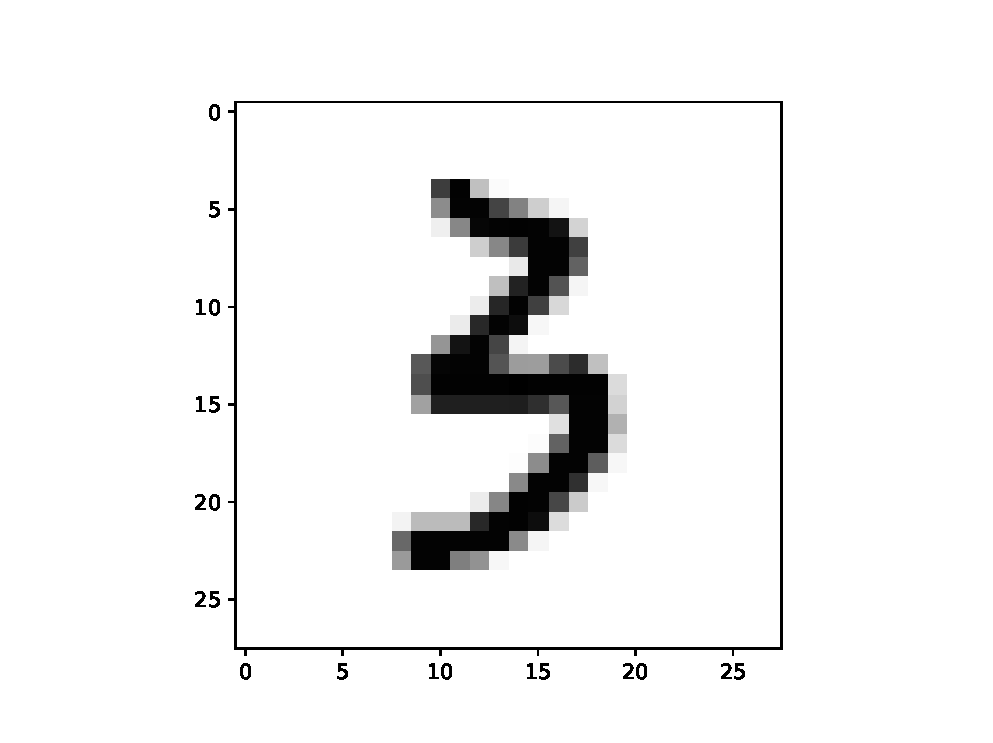
\includegraphics[scale=0.5]{figures/mimic3.eps}}
	\subfloat[Persistence Diagram of the mimic image]{
	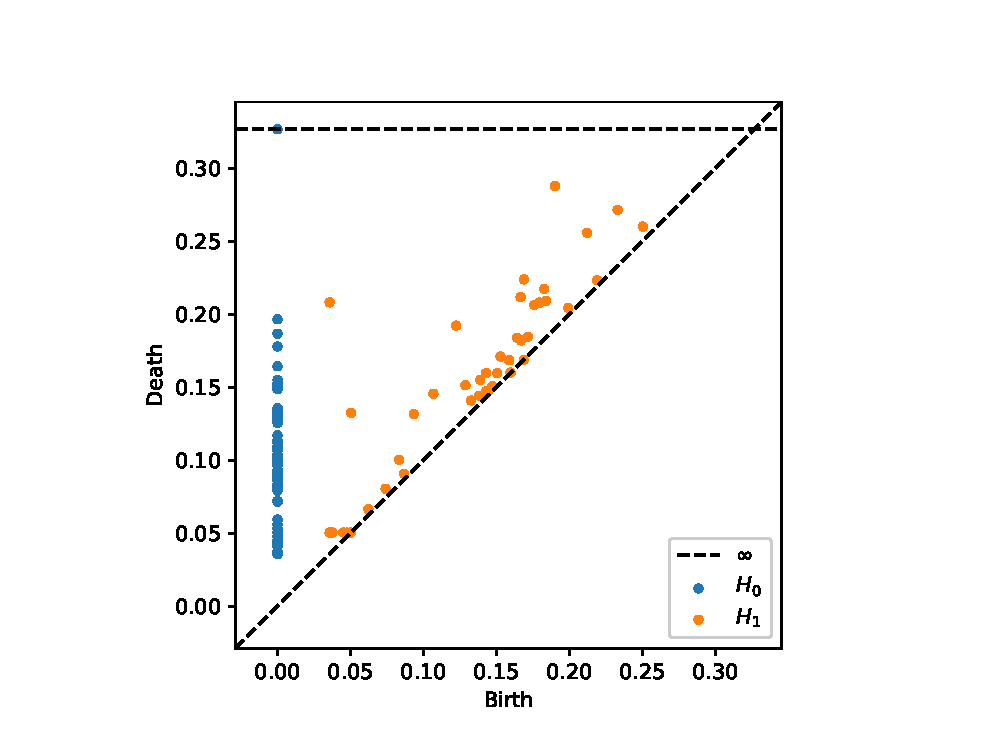
\includegraphics[scale=0.5]{figures/persdgm_mimic3.eps}}
	\\
	\subfloat[Adversarial Image, results in classification as 6]{
	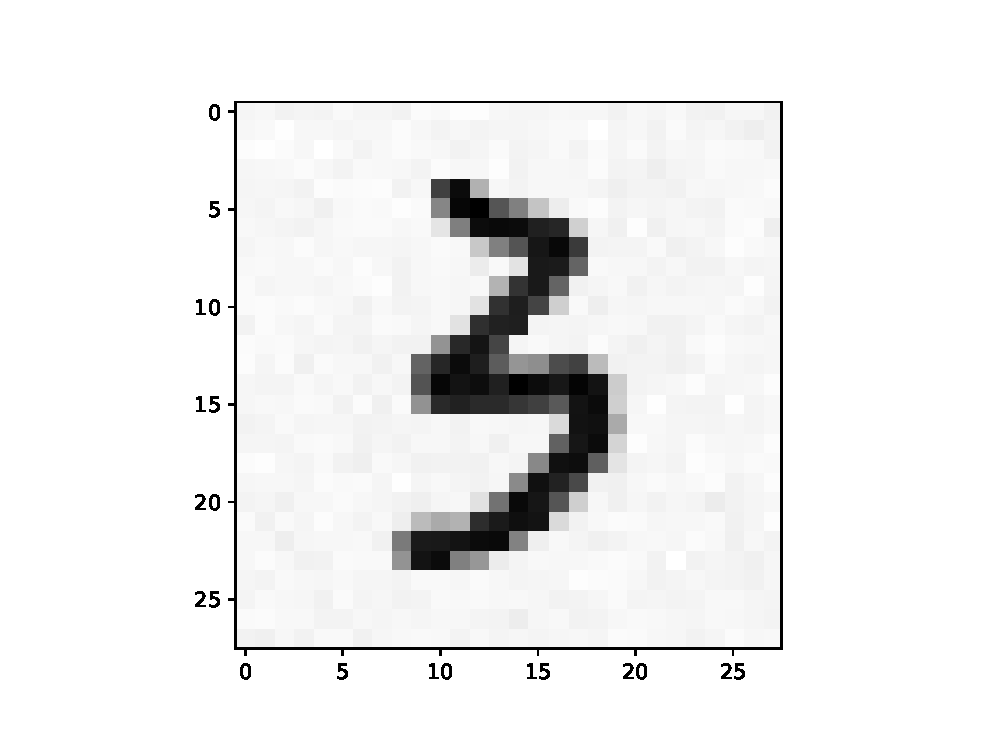
\includegraphics[scale=0.5]{figures/adversarial3.eps}}
	\subfloat[Persistence Diagram of the adversarial image]{
	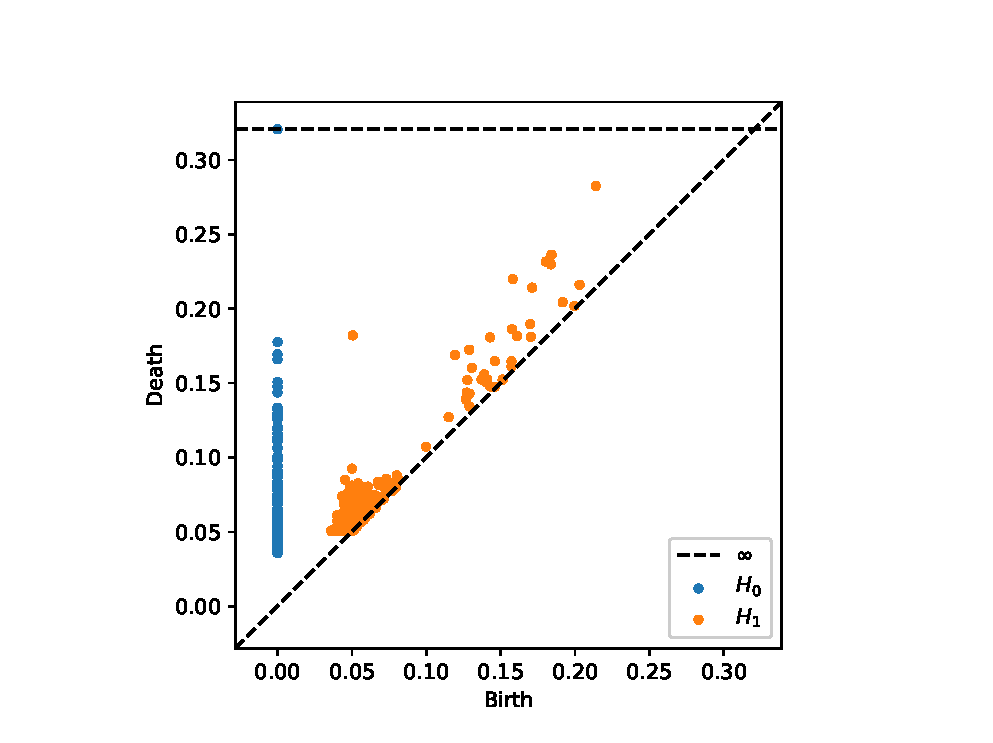
\includegraphics[scale=0.5]{figures/persdgm_adversarial3.eps}}
	\\
	\subfloat[$(\mu=0,\sigma^2=0.05)$ Gaussian Noise added]{
	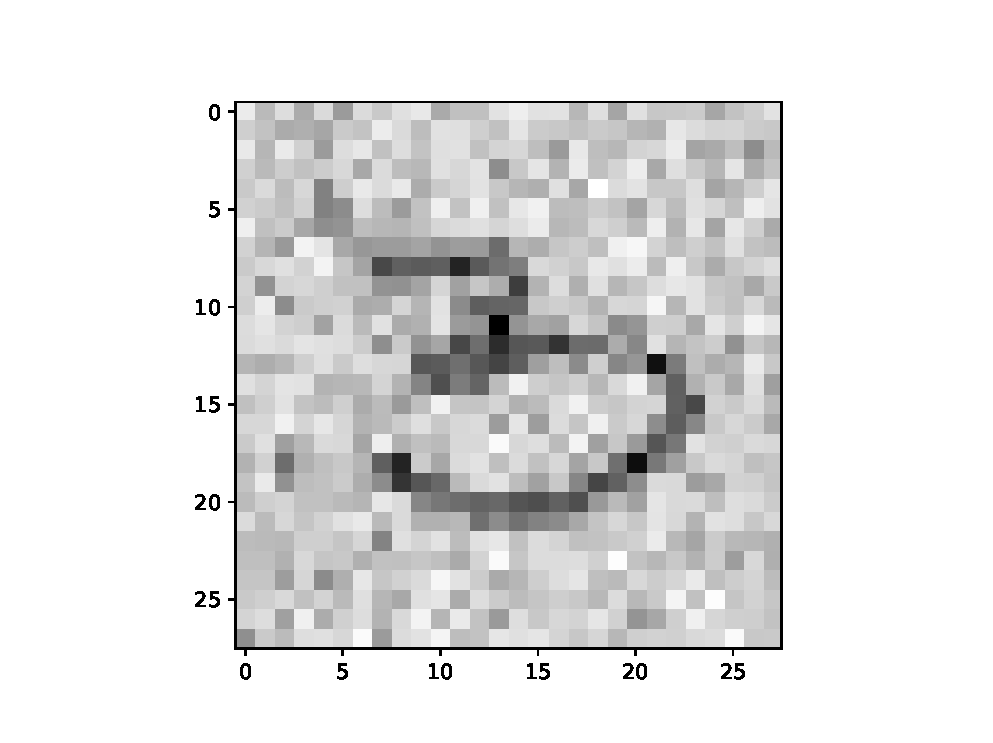
\includegraphics[scale=0.5]{figures/noisy3.eps}}
	\subfloat[Persistence Diagram of the noisy image]{
	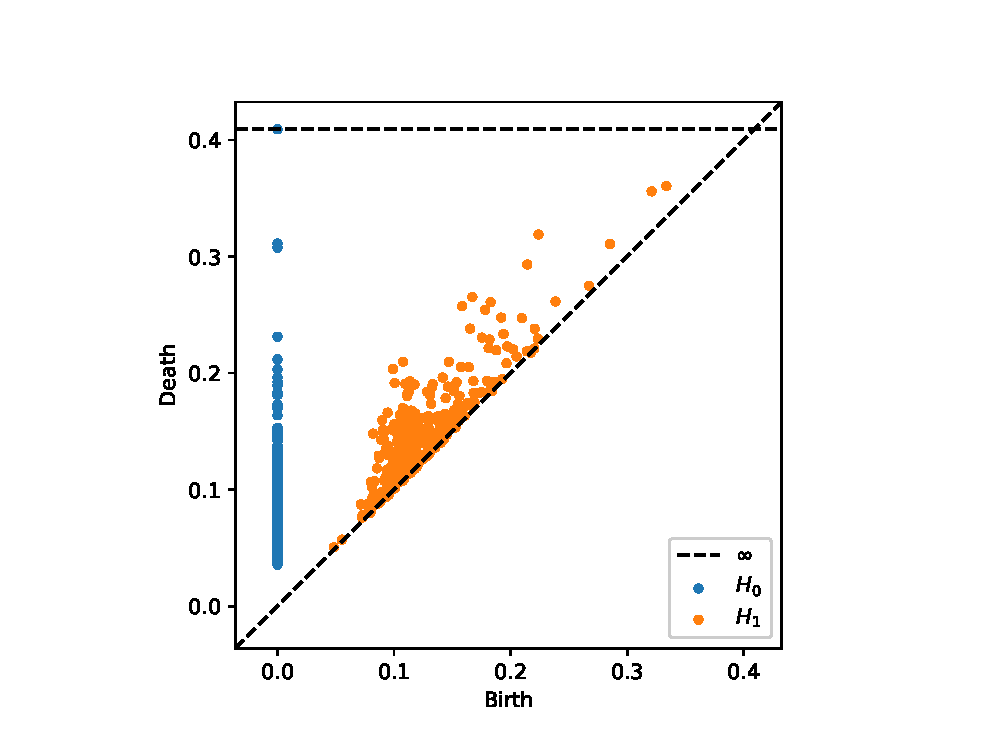
\includegraphics[scale=0.5]{figures/persdgm_noisy3.eps}}
	
	\caption{TEST}
\end{figure*}

\section{Results}

From our experiments, we found that


%------------------------------------------------

\section{Conclusion and Discussion}

Despite yielding some interesting results, our work leaves a lot to be desired. The results may appear compelling to the human eye, but more rigorous methods are needed to determine whether or not there is a significant difference between the persistence diagrams of the adversarial images.



%----------------------------------------------------------------------------------------
%	REFERENCE LIST
%----------------------------------------------------------------------------------------

\begin{thebibliography}{99} % Bibliography - this is intentionally simple in this template

\bibitem[1]{goodfellow2014}
Goodfellow et al.
\newblock Explaining and Harnessing Adversarial Examples. 2014.
\newblock {\em International Conference on Learning Representations}, https://arxiv.org/abs/1412.6572

\bibitem[2]{szegedy2013}
Szegedy et al.
\newblock Intriguing properties of neural networks. 2013.
\newblock {\em International Conference on Learning Representations}, http://arxiv.org/abs/1312.6199
 

 
 
\end{thebibliography}

%----------------------------------------------------------------------------------------

\end{document}
